\chapter{วิธีการดำเนินการวิจัย}
\label{chapter:experiment}

\section{ข้อสมมติฐาาน}
สมมติฐานของงานวิจัยนี้ คือ แบบจำลองการเรียนรู้เชิงลึกที่นำเสนอจะสามารถจัดการปัญหาความไม่สมดุลกันของข้อมูลได้อย่างมีประสิทธิภาพ

\section{การทำการทดลอง}
\subsection{ชุดข้อมูล}
เพื่อที่จะได้ผลการทดลองที่สามารถเปรียบประสิทธิภาพของเทคนิคการแก้ปัญหา จำเป็นจะต้องใช้ชุดข้อมูลที่หลากหลาย โดยแบ่งออกเป็นชุดข้อมูลที่มีความสมดุลและไม่สมดุลกันของข้อมูล ดังนี้

\begin{itemize}
  \item CelebFaces Attributes Dataset (CelebA) \cite{dataset:celebA} ชุดข้อมูลนี้มีความไม่สมดุลกันของข้อมูล ที่ซึ่งเป็นชุดข้อมูลขนาดใหญ่ที่ประกอบไปด้วยภาพหน้าของคนมีชื่อเสียงกว่า 1 หมื่นคน และมีจำนวนภาพมากกว่า 2 แสนภาพ โดยภาพจะมีลักษณะเป็นท่าทางของหน้าและพื้นหลังที่หลากหลายดังรูปที่ \ref{fig:dataset:celebA-1} CelebA นั้นมีคำอธิบายประกอบ (Annotation) ที่หลากหลายมาก เช่น คำอธิบายประกอบที่บอกว่าคนในภาพคือใคร และกำลังยิ้มอยู่หรือไม่ เป็นต้น
  
\begin{figure}[h]
    \centering
    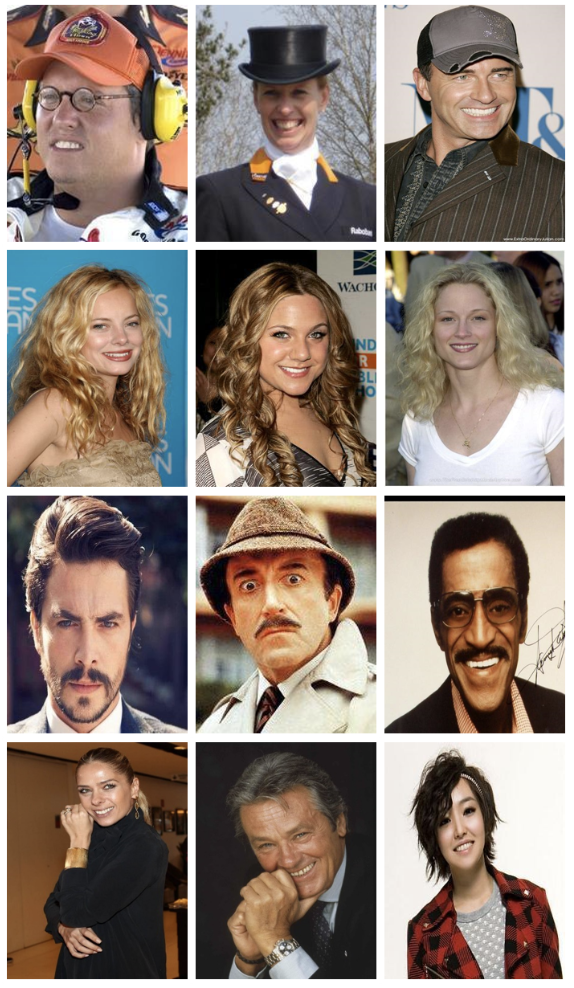
\includegraphics[scale=0.5]{celebA-1}
    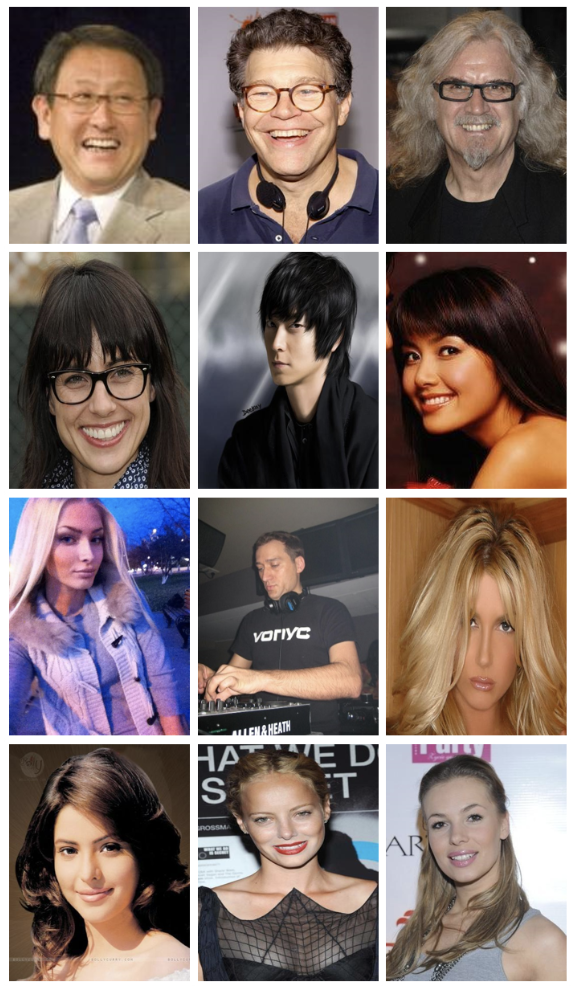
\includegraphics[scale=0.5]{celebA-2}
    \caption{ภาพตัวอย่างของชุดข้อมูล CelebA}
    \label{fig:dataset:celebA-1}
\end{figure}

  \item Cow \cite{dataset:cow} ชุดข้อมูลนี้มีความไม่สมดุลกันของข้อมูล ที่ซึ่งเป็นชุดข้อมูลประเภทวิดีโอ ที่ซึ่งแสดงการเป็นอยู่ของวัวในคอก โดยชุดข้อมูลถูกเก็บจากคอกวัวภายในฟาร์มโชคชัยด้วยกล้องวิดีโอ วิดีโอได้ถูกนำมาแปลงเป็นภาพเฟรม โดยภาพจะมีลักษณะเป็นภาพที่ถ่ายจากมุมบนดังรูปที่ \ref{fig:dataset:cow-1} คำอธิบายประกอบสำหรับชุดข้อมูลนี้ คือ การแสดงพฤติกรรมเป็นสัดของวัวแต่ละตัวในแต่ละเฟรม เช่น ในเฟรมที่ 5 วัว A แสดงพฤติกรรมเป็นสัด วัว B ไม่แสดงพฤติกรรมเป็นสัด และวัว C แสดงพฤติกรรมเป็นสัด เป็นต้น โดยจำนวนเฟรมที่วัวแต่ละตัวไม่แสดงพฤติกรรมเป็นสัดมีจำนวนมากกว่าที่แสดงพฤติกรรมเป็นสัด
  
  \begin{figure}[h]
    \centering
    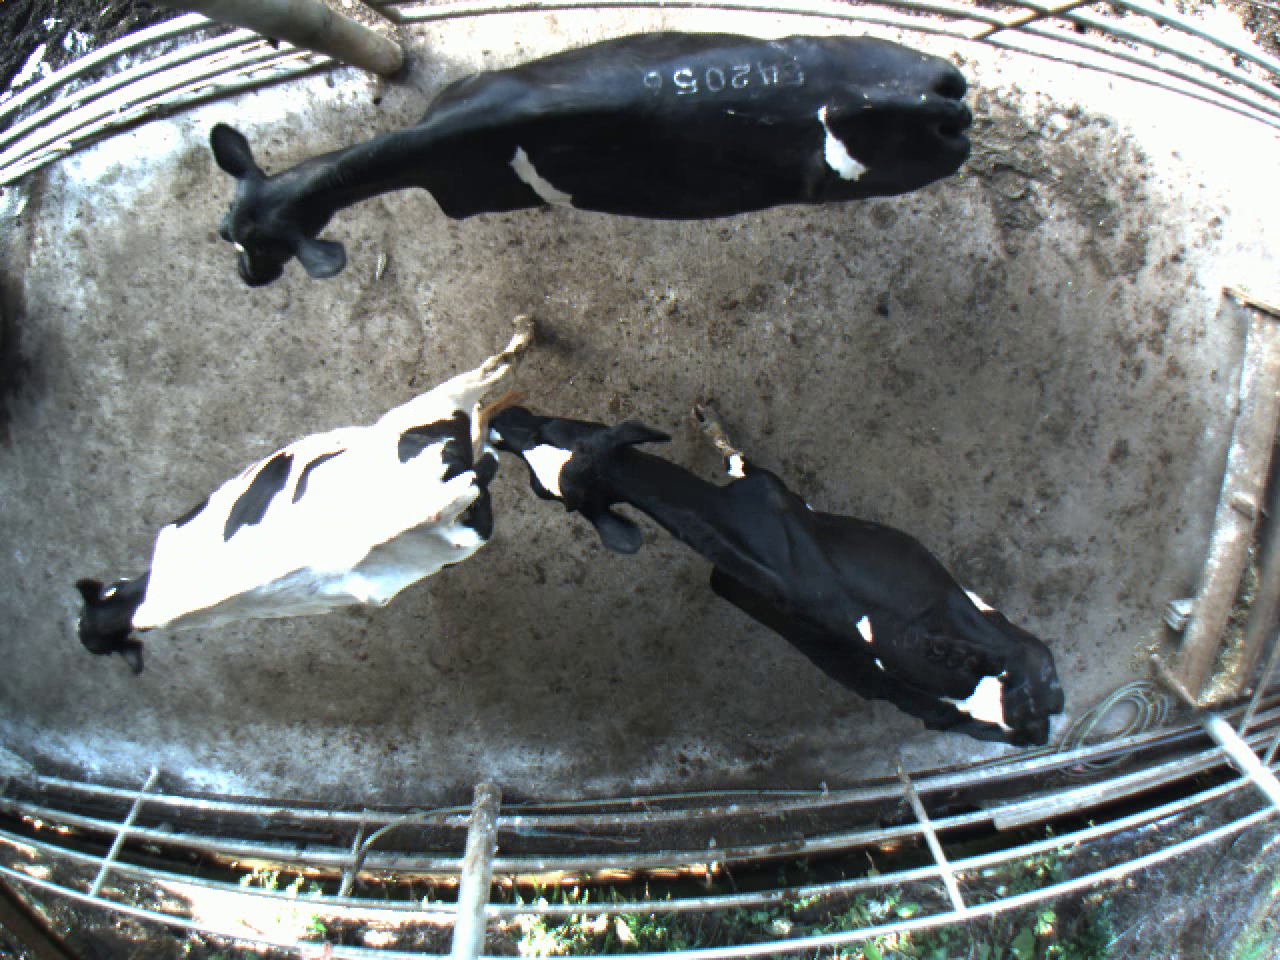
\includegraphics[scale=0.25]{cow-1}
    \caption{ภาพตัวอย่างของชุดข้อมูล Cow}
    \label{fig:dataset:cow-1}
\end{figure}

  \item CIFAR-10 \cite{dataset:cifar-10} ชุดข้อมูลนี้มีความสมดุลกันของข้อมูล ที่ซึ่งเป็นชุดข้อมูลที่ประกอบไปด้วยภาพของสัตว์และยานพาหนะดังรูปที่ \ref{fig:dataset:cifar-1} โดยแบ่งออกเป็นยานพาหนะ 4 ประเภท คือ เครื่องบิน รถยนต์ เรือ และรถบรรทุก และสัตว์ 6 ประเภท คือ นก แมว กวาง หมา กบ และม้า ซึ่งแต่ละประเภทมีจำนวน 6,000 ภาพเท่ากัน รวมทั้งหมดเป็น 6 หมื่นภาพ คำอธิบายประกอบของชุดข้อมูลนี้ คือ ประเภทของภาพ
  
    \begin{figure}[h]
    \centering
    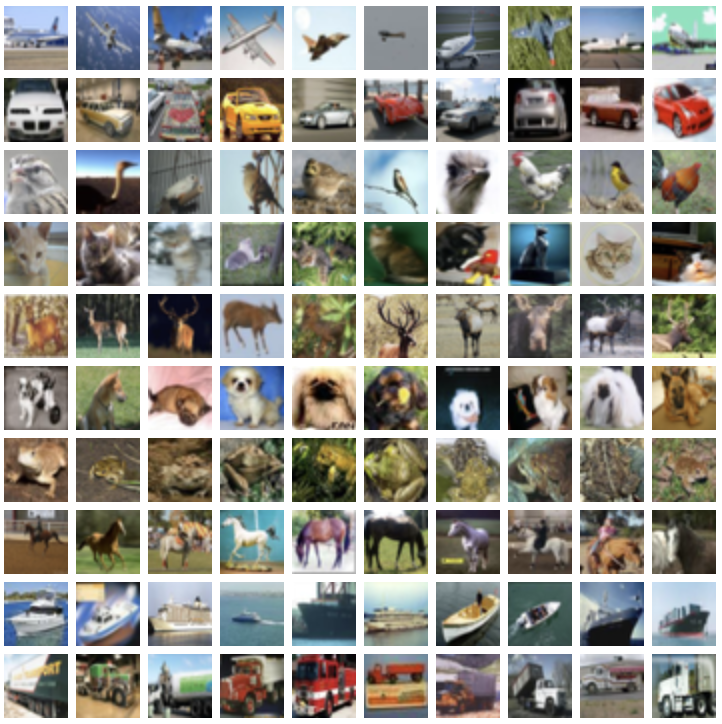
\includegraphics[scale=0.9]{cifar-1}
    \caption{ภาพตัวอย่างของชุดข้อมูล CIFAR-10}
    \label{fig:dataset:cifar-1}
\end{figure}

\end{itemize}
